\section{Variable Length Masked Diffusions: Training}
\label{sec:FlexMDM_informal}

\begin{figure}[t]
\centering
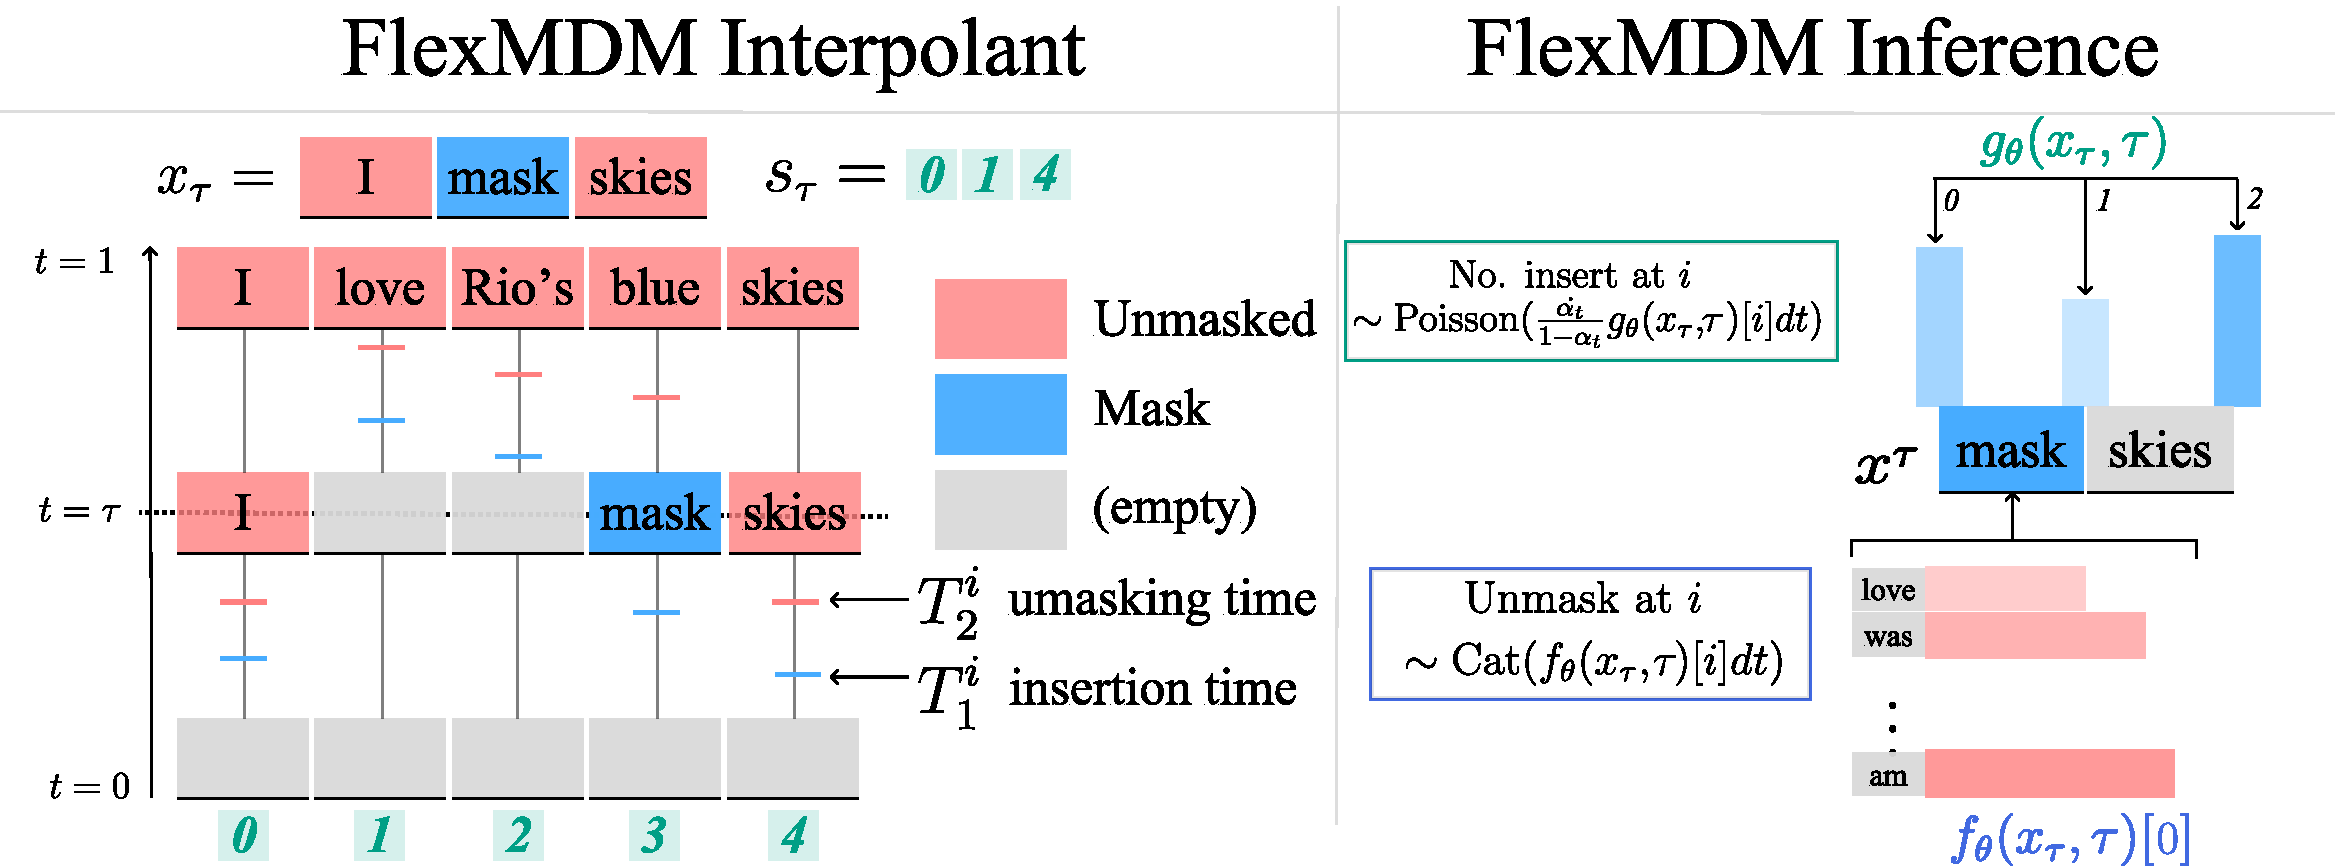
\includegraphics[width=\textwidth,trim={0 0 0 3.5cm}]{Figures/flexmdm_new.pdf}
\caption{\textbf{Left (FlexMDM interpolant).} To draw a sample $x_t$, one can equivalently draw a sample $x_1 \sim p_1$, and for each token \coloredul{xred}{unmask}, \coloredul{xblue}{mask}, or \coloredul{xslategray}{remove} it according to the unmasking and insertion times $(T_1^i, T_2^i)$. An auxiliary interpolant $s_t$ gives closed-form expressions for the FlexMDM rate matrices. \textbf{Right (FlexMDM Inference).} Learned \coloredul{xblue}{unmasking posterior} and \coloredul{xxgreen}{insertion expectation} are later used at inference.}
\label{fig:flexmdm_overview}
\vskip -1.0\baselineskip
\end{figure}

In this section, we introduce \coloredhl{xxpurple}{\textbf{Flexible Length Masked Diffusion Model}} (FlexMDM): a discrete diffusion that models a distribution $p_1$ assigning probabilities to sequences of different lengths. Following the MDM's recipe, we aim to introduce a stochastic interpolant $x_t$ whose marginal distribution defines the path $\{p_t\}_{t\in[0,1]}$ and learn the corresponding CTMC. Everything hinges on selecting an interpolant that is \textbf{(a)} easy to sample at $t=0$ and \textbf{(b)} equipped with a closed-form rate matrix amenable to neural network training.

\textbf{Challenge.} Reusing the MDM interpolant is \emph{inadequate}: at $t=0$, the base distribution $p_0$ would consist of fully-masked sentences of \emph{variable lengths}, which is impossible to sample since we do not know the length statistics of $p_1$ in advance. On the other hand, one can consider an interpolant constructed by masking and removing tokens from a clean sequence. However, this \emph{complicates} the rate matrix characterization--token indices shift as insertions occur. To bridge this gap, we introduce the \coloredhl{xxpurple}{joint interpolant}, an extension of the stochastic interpolant that augments the process with an auxiliary variable explicitly tracking token positions.
This enlarged state space allows us to construct a broader class of rate matrices while preserving an easy-to-sample base distribution.

\textbf{Design of distribution path.} 
We now introduce our FlexMDM's joint interpolant that allows us to model the variable length $p_1$. This construction relies on \emph{two} smooth, monotone schedules \--- an insertion schedule $\alpha \colon [0,1]\to [0,1]$ and an unmasking schedule $\beta \colon [0,1] \to [0,1]$, with the boundary conditions $(\alpha_0,\alpha_1)=(\beta_0,\beta_1)=(0,1)$ and time derivatives denoted by $\dot{\alpha}_t,\dot{\beta}_t$.

To draw $x_t$, we first sample a clean sentence $x_1 \sim p_1$. Independently for each coordinate $i$, we draw an \coloredhl{xxgreen}{insertion time} $T_1^i$ and an \coloredhl{xblue}{unmasking time} $T_2^i$ with $T_1^i < T_2^i$ according to the density below. Accordingly, we either \coloredul{xred}{unmask}, \coloredul{xblue}{mask}, or \coloredul{xslategray}{remove} $x_1^i$ to obtain $x_t^i$:
\begin{align} \label{eqn::FlexMDM_interpolant}T_1^i \sim \dot{\alpha_t} \; dt, & \quad \quad T_2^i \sim \mathbf{1}_{\{t \ge T_1^i\}}\frac{\dot{\beta_t}}{1-\beta_{T_1}} \; dt, \quad  x_t^i = \begin{cases}
        \text{(empty)}, & 0 < t < T_1^i \\
        \mask, & T_1^i \leq t <  T_2^i \\
        x_1^i, &   T_2^i \leq t \leq 1
    \end{cases}
\end{align} 
Here, $\mathbf{1}$ denotes the indicator function. We obtain $x_t$ by concatenating the symbols $x_t^i$, and dropping $x_t^i=\text{(empty)}$. Consequently, the length of $x_t$ is equal to or less than that of $x_1$\footnote{Writing $x_t^i$ to mean the symbol derived from source position $i$ is this a mild abuse of notation since the superscript $i$ refers to a position in $x_1$ rather than a valid index of the (shorter) sequence $x_t$.}  (see Figure~\ref{fig:flexmdm_overview}, left). 
As we mentioned above, we augment $x_t$ with an index-tracking variable $s_t$, forming the joint interpolant $(x_t,s_t)$. Let $\mathrm{len}(x_t)$ denote the length of $x_t$; then
\begin{equation*}
    s_t \colon= \{i \in \{0,\dots,\mathrm{len}(x_1)-1\} \mid T_1^i \le t\},
\end{equation*}
i.e., the set of indices whose clean tokens have \emph{not} been deleted. Equivalently, the positions in $x_1$ referenced by $x_t$'s each index. By regarding $s_t$ as a list and ordering its elements in ascending order, we also have $x_t=(x_1^{s_t[0]},\dots,x_1^{s_t[\mathrm{len}(s_t)-1]})$. We revisit $s_t$ shortly to show how it enables an explicit rate matrix.   Since $(x_t,s_t)$ is governed by the sampled unmasking and insertion times, we write $(x_t,s_t)\sim p_t(\cdot \mid x_1)$. Marginalizing $p_t(\cdot \mid x_1)$ over $x_1 \sim p_1$ yields $p_t$. Since the boundary condition sets $\alpha_0=\beta_0=0$, all tokens are deleted at $t=0$; $p_0$ is the point mass on the empty string.

\textbf{FlexMDM training.} 
We now explain how we train our FlexMDM to learn the desired rate matrix. We first discuss what the CTMC looks like at a high level: 
recall from \eqref{eqn::FlexMDM_interpolant} that when $t$ \emph{increases}, tokens are progressively inserted and unmasked. Indeed, one can show that a CTMC that generates the interpolant can be characterized by two quantities that govern the rate of insertion and unmasking:
\begin{itemize}[leftmargin=*,itemsep=0pt,topsep=0pt]  
  \item \coloredhl{xblue}{Unmasking posterior} (modeled by \xblue{$f_\theta(x,t)[i] \in \Delta(\Sigma)$}): for each index $i$ that $x^i=\mask$, the posterior distribution over the underlying clean token.
  \item \coloredhl{xxgreen}{Insertion expectation} (modeled by \xxgreen{$g_\theta(x,t)[i] \in \mathbb R_{\geq 0}$}): for all indices $i$ in $x$, the expected number of tokens that remain to be inserted in between $x^{i-1}$ and $x^{i}$. 
\end{itemize}
$f_\theta$ resembles the familiar unmasking posterior from MDMs,  
whereas $g_\theta$ is new: it predicts how many tokens need to be inserted. Intuitively, modeling a \emph{variable-length} $p_1$ is harder than the fixed-length setup of MDM--introducing an \coloredhl{xxgreen}{insertion expectation} allows us to parameterize more complicated CTMC for FlexMDM; its rate matrix will appear soon in Proposition~\ref{prop:FlexMDM-rate}. To define the training loss, we set the boundary values of $s_t$ as $s_t[-1]:=-1$ and $s_t[\mathrm{len}(s_t)]:=\mathrm{len}(x_1)$, and let $\phi(x,y)=y-x\log y$ denote a scalar Bregman divergence.
% 
{\small \begin{equation} \label{eq:FlexMDM_loss}
\mathcal{L}_\theta=-\int_{0}^1 \mathbb{E}\underbrace{\Bigg[\frac{\dot{\beta}_t}{1-\beta_t} \sum_{i \colon x_t^i = \mask}\xblue{\log f_\theta(x_t,t)[i,x_1^{s_t[i]}]}}_{\xblue{\text{\emph{unmasking loss}}}} + \underbrace{\frac{\dot{\alpha}_t}{1-\alpha_t}\sum_{i=0}^{\mathrm{len}(x_t)} \phi(s_t[i]-s_t[i-1]-1,\xxgreen{g_\theta(x_t,t)[i]})}_{\xxgreen{\text{\emph{insertion loss}}}}\Bigg]dt.
\end{equation}}
\noindent Here, the expectation is taken over $x_1 \sim p_1$,  $(x_t, s_t) \sim p_t(\cdot | x_1)$. Proposition~\ref{prop:FlexMDM-loss} exactly characterizes the unmasking posterior and insertion expectation and shows they uniquely minimize \eqref{eq:FlexMDM_loss}.

\begin{proposition}[FlexMDM training loss]   \label{prop:FlexMDM-loss}
The loss $\mathcal{L}_\theta$ in \eqref{eq:FlexMDM_loss} is uniquely minimized at
\begin{equation*}
    \xblue{f_\theta(x, t)[i, v]} = \underbrace{\mathbb{P} (x_1^{s_t[i]} = v | x_t = x)}_{\xblue{\text{unmasking posterior}}}, \quad \xxgreen{g_\theta(x, t)[i]} = \underbrace{\mathbb{E}[s_t[i] - s_t[i-1] - 1 | x_t = x]}_{\xxgreen{\text{insertion expectation}}}.
\end{equation*}
\end{proposition}
These quantities match the explanation above: the posterior over the clean token together with the expected number of insertions. They precisely determine the FlexMDM rate matrix stated next.
\begin{proposition}[FlexMDM Rate Matrix] \label{prop:FlexMDM-rate}
Let the rate matrix $R_t$ be defined as:
\begin{equation}
\begin{aligned} \label{eq:rate_FlexMDM}
\text{\coloredhl{xblue}{Unmask}}& :R_t\left(x, \replaceat{x}{i}{v}\right)
    = \tfrac{\dot{\beta}_t}{1 - \beta_t} \cdot \mathbb{P}(x_1^{s_t[i]}=v | x_t=x),\quad v \in \Sigma, x^i =\mask \\
    \text{\coloredhl{xxgreen}{Insert}}&: R_t\left(x, \insertat{x}{i}{\mask}\right)
    = \tfrac{\dot{\alpha}_t}{1 - \alpha_t} \cdot \mathbb{E} \left[s_t[i]-s_t[i-1]-1 | x_t = x\right],  
\end{aligned}
\end{equation}
where $\insertat{x}{i}{\mask}$ is the sequence obtained from $x$ by inserting a mask token in between $(x^{i-1},x^i)$. Then $R_t$ solves the KFE (equation~\eqref{eq:kfe}) with $p_t$ as the probability mass function of the FlexMDM interpolant $x_t$.
\end{proposition}

Proposition~\ref{prop:FlexMDM-loss} thus implies that minimizing the loss yields exact recovery of the rate matrix. In practice, we could simulate the CTMC using the learned networks $(f_\theta,g_\theta)$ in place of the ground-truth quantities in \eqref{eq:rate_FlexMDM}. By denoting the resulting terminal distribution as $p_1^\theta$, the variational loss quantifies the terminal-time KL divergence:
\begin{equation*}
    \mathcal{D}_\mathrm{KL}(p_1 || p_1^\theta) \leq \mathcal{L_\theta} - \mathcal{L}_\star
\end{equation*}
We defer formal demonstration of propositions and the KL divergence guarantee to Appendix~\ref{sec:app-joint-interpolant-flex-mdm}. Definition of the joint interpolant is reinstated in definition \ref{def:flexmdm-interpolant-def-appendix}, the rate matrix in proposition \ref{prop:appendix-flexmdm-rate}, the loss and variational bound in proposition \ref{prop:flexmdm-loss-appendix}.

\textbf{Remark.}
Our FlexMDM interpolant introduces only one extra quantity beyond MDM's unmasking posterior: the insertion expectation, a simple scalar per position. This stems from our design choice to gradually insert and then unmask a token. As shown in Section~\ref{sec:experiment_llada}, this enables efficient task transfer of pretrained MDM weights. In contrast, alternative interpolants would require modeling more complex objects, such as a full token distribution, adding unnecessary training burden.
